\documentclass[a4paper,11pt,fleqn,dvipsnames,twoside,openright]{memoir} 	% Openright aabner kapitler paa hoejresider (openany begge)

%%%% PACKAGES %%%%

% ¤¤ Oversaettelse og tegnsaetning ¤¤ %
\usepackage[utf8]{inputenc}					% Input-indkodning af tegnsaet (UTF8)
\usepackage[danish]{babel}					% Dokumentets sprog
\usepackage[T1]{fontenc}					% Output-indkodning af tegnsaet (T1)
\usepackage{ragged2e,anyfontsize}			% Justering af elementer
\usepackage{fixltx2e}						% Retter forskellige fejl i LaTeX-kernen

																			
% ¤¤ Figurer og tabeller (floats) ¤¤ %
\usepackage{graphicx} 						% Haandtering af eksterne billeder (JPG, PNG, EPS, PDF)
%\usepackage{eso-pic}						% Tilfoej billedekommandoer paa hver side
%\usepackage{wrapfig}						% Indsaettelse af figurer omsvoebt af tekst. \begin{wrapfigure}{Placering}{Stoerrelse}
\usepackage[space]{grffile}					% Bør gøre det muligt at have mellemrum i filnavne.
\usepackage{multirow}                		% Fletning af raekker og kolonner (\multicolumn og \multirow)
\usepackage{multicol}         	        	% Muliggoer output i spalter
\usepackage{rotating}						% Rotation af tekst med \begin{sideways}...\end{sideways}
\usepackage{colortbl} 						% Farver i tabeller (fx \columncolor og \rowcolor)
\usepackage[usenames,dvipsnames]{xcolor}	% Definer farver med \definecolor. Se mere: http://en.wikibooks.org/wiki/LaTeX/Colors
%\usepackage{flafter}						% Soerger for at floats ikke optraeder i teksten foer deres reference
\let\newfloat\relax 						% Justering mellem float-pakken og memoir
\usepackage{float}							% Muliggoer eksakt placering af floats, f.eks. \begin{figure}[H]
\setlength{\heavyrulewidth}{0.15em}			% Sætter \toprule og \bottomrule til fast størrelse (0.08 er default)
%\setlength{\lightrulewidth}{0.05em}		% Sætter \midrule til fast størrelse (0.05 er default)
\usepackage{array}							% Bruges i forbindelse med \newcolumntype-command under egne commands
\usepackage{pdfpages}						% Bruges så der kan indsættes pdf, som sider (se forside for eksempel)
\usepackage{tablefootnote}


% ¤¤ Matematik mm. ¤¤
\usepackage{amsmath,amssymb,stmaryrd} 		% Avancerede matematik-udvidelser
\usepackage{mathtools}						% Andre matematik- og tegnudvidelser
\usepackage{textcomp}                 		% Symbol-udvidelser (f.eks. promille-tegn med \textperthousand )
\usepackage{rsphrase}						% Kemi-pakke til RS-saetninger, f.eks. \rsphrase{R1}
\usepackage[version=3]{mhchem} 				% Kemi-pakke til flot og let notation af formler, f.eks. \ce{Fe2O3}
\usepackage{siunitx}						% Flot og konsistent praesentation af tal og enheder med \si{enhed} og \SI{tal}{enhed}
\sisetup{locale=DE}							% Opsaetning af \SI (DE for komma som decimalseparator) 

% ¤¤ Referencer og kilder ¤¤ %
\usepackage[danish]{varioref}				% Muliggoer bl.a. krydshenvisninger med sidetal (\vref)
\usepackage{natbib}							% Udvidelse med naturvidenskabelige citationsmodeller
\usepackage{xr-hyper}							% Referencer til eksternt dokument med \externaldocument{<NAVN>}
\externaldocument[DokRap-]{../Dokumentationsrapport/Dokumentationsrapport}	% Muliggør eksterne referencer til produktrapporten
%\usepackage{glossaries}					% Terminologi- eller symbolliste (se mere i Daleifs Latex-bog)



% ¤¤ Misc. ¤¤ %
\usepackage{lipsum}							% Dummy text \lipsum[..]
\usepackage[shortlabels]{enumitem}			% Muliggoer enkelt konfiguration af lister
\usepackage{pdfpages}						% Goer det muligt at inkludere pdf-dokumenter med kommandoen \includepdf[pages={x-y}]{fil.pdf}	
\pdfoptionpdfminorversion=6					% Muliggoer inkludering af pdf dokumenter, af version 1.6 og hoejere
\pretolerance=2500 							% Justering af afstand mellem ord (hoejt tal, mindre orddeling og mere luft mellem ord)

% Kommentarer og rettelser med \fxnote. Med 'final' i stedet for 'draft' udloeser hver note en error i den faerdige rapport.
\usepackage[footnote,draft,danish,silent,nomargin]{fixme}		


%%%% CUSTOM SETTINGS %%%%

% ¤¤ Marginer ¤¤ %
\setlrmarginsandblock{3.5cm}{2.5cm}{*}		% \setlrmarginsandblock{Indbinding}{Kant}{Ratio}
\setulmarginsandblock{2.5cm}{3.0cm}{*}		% \setulmarginsandblock{Top}{Bund}{Ratio}
\checkandfixthelayout 						% Oversaetter vaerdier til brug for andre pakker

%	¤¤ Afsnitsformatering ¤¤ %
\setlength{\parindent}{0mm}           		% Stoerrelse af indryk
\setlength{\parskip}{3mm}          			% Afstand mellem afsnit ved brug af double Enter
\linespread{1,1}							% Linie afstand
\newcommand{\tab}{\hspace*{2em}}			% ved \tab{} indrykkes det i klammerne ind
\usepackage{titlesec}							%Muliiggøre ændring af sections i alle lag
\titleformat*{\section}{\LARGE\bfseries\color{NavyBlue}}		%section = størst
\titleformat*{\subsection}{\Large\bfseries\color{RoyalBlue}}		%sub og subsub har samme størrelse
\titleformat*{\subsubsection}{\Large\bfseries}
\titleformat*{\paragraph}{\large\bfseries}		%Benyttes umiddelbart ikke
\titleformat*{\subparagraph}{\large\bfseries}	%Benyttes umiddelbart ikke

% ¤¤ Litteraturlisten ¤¤ %
\bibpunct[,]{[}{]}{;}{a}{,}{,} 				% Definerer de 6 parametre ved Harvard henvisning (bl.a. parantestype og seperatortegn)
\bibliographystyle{bibtex/harvard}			% Udseende af litteraturlisten.

% ¤¤ Indholdsfortegnelse ¤¤ %
\setsecnumdepth{subsubsection}		 			% Dybden af nummerede overkrifter (part/chapter/section/subsection)
\maxsecnumdepth{subsection}					% Dokumentklassens graense for nummereringsdybde
\settocdepth{subsection} 					% Dybden af indholdsfortegnelsen

% ¤¤ Lister ¤¤ %
\setlist{
  topsep=-5pt,								% Vertikal afstand mellem tekst og listen	Default: 0
  itemsep=-1ex,								% Vertikal afstand mellem items
} 

% ¤¤ Visuelle referencer ¤¤ %
\usepackage[colorlinks]{hyperref}			% Danner klikbare referencer (hyperlinks) i dokumentet.
\hypersetup{colorlinks = true,				% Opsaetning af farvede hyperlinks (interne links, citeringer og URL)
    linkcolor = black,
    citecolor = black,
    urlcolor = black
}

% ¤¤ Opsaetning af figur- og tabeltekst ¤¤ %
\usepackage{caption}
\captionnamefont{\small\bfseries\itshape}	% Opsaetning af tekstdelen ('Figur' eller 'Tabel')
\captiontitlefont{\small}					% Opsaetning af nummerering
\captiondelim{. }							% Seperator mellem nummerering og figurtekst
\hangcaption								% Venstrejusterer flere-liniers figurtekst under hinanden
\captionsetup{width=\linewidth,labelfont={bf,it}}
\setlength{\abovecaptionskip}{-1pt}			% Afstand over figurteksten
\setlength{\belowcaptionskip}{-12pt}			% Afstand under figurteksten
		
% ¤¤ Navngivning ¤¤ %
\addto\captionsdanish{
	\renewcommand\appendixname{Appendiks}
	\renewcommand\contentsname{Indholdsfortegnelse}	
	\renewcommand\appendixpagename{Appendiks}
	\renewcommand\appendixtocname{Appendiks}
	\renewcommand\cftchaptername{\chaptername~}				% Skriver "Kapitel" foran kapitlerne i indholdsfortegnelsen
	\renewcommand\cftappendixname{\appendixname~}			% Skriver "Appendiks" foran appendiks i indholdsfortegnelsen
}

% ¤¤ Kapiteludssende ¤¤ %
\definecolor{chapnumcolor}{RGB}{23,54,93}		% Definerer en farve til brug til kapiteludseende
\definecolor{chapfontcolor}{RGB}{29,69,118}
\newif\ifchapternonum

\makechapterstyle{jenor}{					% Definerer kapiteludseende frem til ...
  \renewcommand\beforechapskip{0pt}
  \renewcommand\printchaptername{}
  \renewcommand\printchapternum{}
  \renewcommand\printchapternonum{\chapternonumtrue}
  \renewcommand\chaptitlefont{\fontfamily{pbk}\fontseries{db}\fontshape{n}\fontsize{25}{35}\selectfont\raggedleft\color{chapfontcolor}}
  \renewcommand\chapnumfont{\fontfamily{pbk}\fontseries{m}\fontshape{n}\fontsize{1in}{0in}\selectfont\color{chapnumcolor}}
  \renewcommand\printchaptertitle[1]{%
    \noindent
    \ifchapternonum
    \begin{tabularx}{\textwidth}{X}
    {\let\\\newline\chaptitlefont ##1\par} 
    \end{tabularx}
    \par\vskip-2.5mm\hrule
    \else
    \begin{tabularx}{\textwidth}{Xl}
    {\parbox[b]{\linewidth}{\chaptitlefont ##1}} & \raisebox{-15pt}{\chapnumfont \thechapter}
    \end{tabularx}
    \par\vskip2mm\hrule
    \fi
  }
}											% ... her

\chapterstyle{jenor}						% Valg af kapiteludseende - Google 'memoir chapter styles' for alternativer

% ¤¤ Sidehoved ¤¤ %

\makepagestyle{AAU}							% Definerer sidehoved og sidefod udseende frem til ...
\makepsmarks{AAU}{%
	\createmark{chapter}{left}{shownumber}{}{. \ }
	\createmark{section}{right}{shownumber}{}{. \ }
	\createplainmark{toc}{both}{\contentsname}
	\createplainmark{lof}{both}{\listfigurename}
	\createplainmark{lot}{both}{\listtablename}
	\createplainmark{bib}{both}{\bibname}
	\createplainmark{index}{both}{\indexname}
	\createplainmark{glossary}{both}{\glossaryname}
}
\nouppercaseheads											% Ingen Caps oenskes

\makeevenhead{AAU}{Printer booking}{}{\leftmark}					% Definerer lige siders sidehoved (\makeevenhead{Navn}{Venstre}{Center}{Hoejre})
\makeoddhead{AAU}{\rightmark}{}{Ingeniørhøjskolen, Aarhus Universitet}		% Definerer ulige siders sidehoved (\makeoddhead{Navn}{Venstre}{Center}{Hoejre})
\makeevenfoot{AAU}{\thepage}{}{}							% Definerer lige siders sidefod (\makeevenfoot{Navn}{Venstre}{Center}{Hoejre})
\makeoddfoot{AAU}{}{}{\thepage}								% Definerer ulige siders sidefod (\makeoddfoot{Navn}{Venstre}{Center}{Hoejre})
\makeheadrule{AAU}{\textwidth}{0.5pt}						% Tilfoejer en streg under sidehovedets indhold
\makefootrule{AAU}{\textwidth}{0.5pt}{1mm}					% Tilfoejer en streg under sidefodens indhold

\copypagestyle{AAUchap}{AAU}								% Sidehoved for kapitelsider defineres som standardsider, men med blank sidehoved
\makeoddhead{AAUchap}{}{}{}
\makeevenhead{AAUchap}{}{}{}
\makeheadrule{AAUchap}{\textwidth}{0pt}
\aliaspagestyle{chapter}{AAUchap}							% Den ny style vaelges til at gaelde for chapters
															% ... her
															
\pagestyle{AAU}												% Valg af sidehoved og sidefod





%%%% CUSTOM COMMANDS %%%%

% ¤¤ Billede hack ¤¤ %
\newcommand{\figur}[4]{
		\begin{figure}[H] \centering
			\includegraphics[width=#1\textwidth]{Billeder/#2}
			\caption{#3}\label{#4}
		\end{figure} 
}


% ¤¤ Venstre orienterer al tekst i p{Ycm} ¤¤ %
\newcolumntype{x}[1]{%
>{\raggedright\hspace{0pt}}p{#1}}

% ¤¤ Newline til x{} ¤¤ %
% \\ virker åbenbart ikke når man selv laver en columntype... :(
\newcommand{\tn}{\tabularnewline}


% ¤¤ Pæn opsætning af titelblad-dele ¤¤ %
% ¤¤ Husk at ændre dato i senere projekter ¤¤ %
\newcommand{\titelblad}[2]{
\begin{tabular}[ht]{x{7cm}x{7cm}}
\textbf{Navn: } #1		&\textbf{Studienummer: } #2	\tn
\textbf{Dato} 31-05-2013	\tn
\multicolumn{2}{l}{\textbf{Underskrift: }\line(1,0){340}}
\end{tabular}
}


% ¤¤ Specielle tegn ¤¤ %
\newcommand{\grader}{^{\circ}\text{C}}
\newcommand{\gr}{^{\circ}}
\newcommand{\g}{\cdot}


%%%% ORDDELING %%%%

\hyphenation{}

%%%Indsat af Søren%%%
\usepackage{listings}
\usepackage{color}
 
\definecolor{dkgreen}{rgb}{0,0.6,0}
\definecolor{gray}{rgb}{0.5,0.5,0.5}
\definecolor{mauve}{rgb}{0.58,0,0.82}
 
\lstset{ %
  language=Octave,                % the language of the code
  basicstyle=\footnotesize,           % the size of the fonts that are used for the code
  numbers=left,                   % where to put the line-numbers
  numberstyle=\tiny\color{gray},  % the style that is used for the line-numbers
  stepnumber=2,                   % the step between two line-numbers. If it's 1, each line 
                                  % will be numbered
  numbersep=5pt,                  % how far the line-numbers are from the code
  backgroundcolor=\color{white},      % choose the background color. You must add \usepackage{color}
  showspaces=false,               % show spaces adding particular underscores
  showstringspaces=false,         % underline spaces within strings
  showtabs=false,                 % show tabs within strings adding particular underscores
  frame=single,                   % adds a frame around the code
  rulecolor=\color{black},        % if not set, the frame-color may be changed on line-breaks within not-black text (e.g. comments (green here))
  tabsize=2,                      % sets default tabsize to 2 spaces
  captionpos=b,                   % sets the caption-position to bottom
  breaklines=true,                % sets automatic line breaking
  breakatwhitespace=false,        % sets if automatic breaks should only happen at whitespace
  title=\lstname,                   % show the filename of files included with \lstinputlisting;
                                  % also try caption instead of title
  keywordstyle=\color{blue},          % keyword style
  commentstyle=\color{dkgreen},       % comment style
  stringstyle=\color{mauve},         % string literal style
  escapeinside={\%*}{*)},            % if you want to add LaTeX within your code
  morekeywords={*,...},              % if you want to add more keywords to the set
  deletekeywords={...}              % if you want to delete keywords from the given language
}				% Preamble indlaeses
\raggedbottom									% Soerger for at LaTeX ikke "straekker" teksten


\begin{document}									% Starter dokumentet - obligatorisk
\frontmatter										% Forindhold - nummereres med romertal


\cleardoublepage	% Indsaetter tom side, saa naeste kapitel starter paa hoejre side (hvis noedvendigt)

\include{Kapitler/Pre_ToC/pre_ToC}
\cleardoublepage

%Revision history and glossary comes before table of contents
%%%%%%%% Forside arkitektur  %%%%%%%%
%\title{	\normalsize \textsc{Aarhus School of Engineering} 	% Subtitle of the document
%		 	\\[2.0cm]													% 2cm spacing
%			\HRule{0.5pt} \\										% Upper rule
%			\Huge \textbf{Concept of Operations}\ref{fig:sd}	% Title
%			\HRule{2pt} \\ [0.2cm]								% Lower rule + 0.5cm spacing
%			\normalsize SitaWare Civilian \\ Company: B									% Todays date
%		}

\frontpagetitle{Aarhus School of Engineering}{System Engineering Management Plan}{SitaWare Civilian}{Company: B}
		

%\author{
%		John F. Doe\\	
%		Imaginary University of Examples\\	
%		Made up department of Randomness\\
%        \texttt{your@email.com} \\
%}

\thispagestyle{empty}		% Remove page numbering on this page

%\printtitle			% Print the title data as defined above
~\\
~\\
~\\
~\\
~\\
~\\
~\\
~\\
~\\
~\\
~\\
~\\
~\\

\subsection*{Development Team}
\titelbladstuderende{Jens Kuhr Jørgensen}{11690@iha.dk} \\
\titelbladstuderende{Thomas Fiil Lyngholm}{11641@iha.dk} \\
\titelbladstuderende{Rasmus Fredensborg Jensen}{11471@iha.dk} \\
\titelbladstuderende{René Arendt Sørensen}{11553@iha.dk} \\
\titelbladstuderende{Kristian Falkesgaard Ørts}{11537@iha.dk} \\
\titelbladstuderende{Jonas Harder Poulsen}{20104025@iha.dk} \\
\titelbladstuderende{Peter Kristian Mathiesen}{11490@iha.dk} \\

\subsection*{Customer}
\titelbladvejleder{Miran Hasanagic}{miran.hasanagic@eng.au.dk} \\
  
%\vfill
%\printauthor			% Print the author data as defined above

\chapter*{Revision history}

\begin{table}[H]  
\centering
\scalebox{1.0}{
\begin{tabular}{|l|l|p{10cm}|}
\multicolumn{3}{l}{}\\\hline
	\textbf{Version}	&\textbf{Date}		&\textbf{Changes}		\\\hline
	0.1		&18-02-2015		&Document created.		\\\hline
	1.0		&23-02-2015		&Document delivery		\\\hline
	1.1		&24-02-2015		&Document revised and edited.		\\\hline
	\textlabel{2.0}{ver:current}		&02-03-2015		&Document delivery.		\\\hline
\end{tabular}}
\caption {Revision history.} 
\label{tab:table_revision} 
\end{table} 

\chapter*{Glossary and Terms}

The following table contains a glossary of abbreviations and technical subject-specifik terms used in this document which require further explanation. 

\begin{table}[H]  
\centering
\scalebox{1.0}{
\begin{tabular}{|l|p{5cm}|p{6cm}|}
\multicolumn{3}{l}{}\\\hline
	\textbf{Abbreviation}	&\textbf{Meaning}		&\textbf{Explanation}		\\\hline
	&&		\\\hline
	\end{tabular}}
\caption {Glossary.} 
\label{tab:table_glossary} 
\end{table}


%%%% Indholdsfortegnelse (TOC) %%%%
\phantomsection									% Kunstigt afsnit, som hyperlinks kan 'holde fast i'
\pdfbookmark[0]{Indholdsfortegnelse}{indhold}	% Tildeler en klikbar bookmark til den endelige PDF
\tableofcontents*								% Indholdsfortegnelsen (kaldet ToC) 


\mainmatter										% Hovedindhold - nummereres fra side 1

\chapter{Introduktion}
test
%Referenced documents
\chapter{Referenced Documents}
This chapter contains a brief description of the documents referenced to in this document.

\begin{table}[H]  
\centering
\scalebox{1.0}{
\begin{tabular}{|l|l|p{6cm}|}
\multicolumn{3}{l}{}\\\hline
	\textbf{Version}	&\textbf{Document name}		&\textbf{Description}		\\\hline
	\textbf{1.3}		& System Requirement Specification		& The System Requirement Specification(SRS) contains all of the requirements that the system has to fulfil. 		\\\hline

\end{tabular}}
\caption {Referenced Documents.} 
\label{tab:table_ReferencedDocuments} 
\end{table} 

\chapter{System-wide Design Decisions}

In this chapter, the decision for the system-wide detailed design is made.
\section{Parts Decisions}
\textbf{The HQ} shall be a stationary post mounted in a mobile vehicle. The HQ shall be implemented on a PC. The user interaction is supposed to be a mix between use of mouse, keyboard and touch screen. It must be possible to give all commands from here. The PC must have a wireless internet connection. To process data the PC must have a processor.\\

\textbf{The Dismounted COP} shall be mounted on the wrist of the user. Therefor the Dismounted COP must be within dimensions of 13x6x1 cm. It must be shock-, water- and heat resistant. The Dismounted COP must have a touch screen which can be used with or without gloves. Furthermore the Dismounted COP must be able to alert the users about radiation, low oxygen levels and dangerous temperatures.\\

\textbf{A Server} shall be used to distribute data between users. It must contain a database for storage of relevant information. The server must also be able to communicate with other SitaWare solutions.\\

For reference purposes the decisions are listed below:
\begin{description}
\item[SDD-0100] The HQ shall be implemented on a PC.
\item[SDD-0110] The PC shall have a Touch screen, to display relevant information and to make user interaction easy.
\item[SDD-0120] The PC shall have a mouse, to make user interaction easy.
\item[SDD-0130] The PC shall have a keyboard, to make user interaction easy.
\item[SDD-0140] The PC shall have a GPS, to get the location of the HQ.
\item[SDD-0150] The PC shall have a Telecommunication module, to access the internet.
\item[SDD-0160] The PC shall have a speaker, to enable audio communication.
\item[SDD-0170] The PC shall have a microphone, to enable audio communication.
\item[SDD-0180] The PC shall have a processor, to process data.
\item[SDD-0200] The system shall have a Dismounted COP.
\item[SDD-0210] The Dismounted COP shall have a GPS, to get the location of the Dismounted COP.
\item[SDD-0220] The Dismounted COP shall have a Micro Controller, to process data.
\item[SDD-0230] The Dismounted COP shall have a Telecommunication module, to access the internet.
\item[SDD-0240] The Dismounted COP shall have a Touch screen, to display relevant information and to make user interaction easy.
\item[SDD-0250] The Dismounted COP shall have a speaker, to enable audio communication.
\item[SDD-0260] The Dismounted COP shall have a microphone, to enable audio communication.
\item[SDD-0270] The Dismounted COP shall have a battery, to be mobile.
\item[SDD-0280] The Dismounted COP shall have a Radiation sensor to alert the user about radiation.
\item[SDD-0290] The Dismounted COP shall have an Oxygen sensor to alert the user about low oxygen levels.
\item[SDD-0299] The Dismounted COP shall have a Temperature sensor to alert the user about dangerous temperatures.
\item[SDD-0300] The system shall have a Server to distribute data.
\item[SDD-0310] The Server shall have a Database to store information.
\end{description}


\chapter{System Architectural Design}
\section{System Components}
This chapter seeks to identify the system components. It provides a block definition diagram (bdd) of the system, where the system components are determined along with the static relationship between them. A unique name has been assigned each block (with prefix SDD (System Design Description)), so that each system component can be mapped to the requirement from which it originates in the Requirements Traceability Matrix in section \ref{chap:req_trace}. The block definition diagram is shown in figure \ref{fig:block_diagram}:
\begin{figure}[H]
\centering
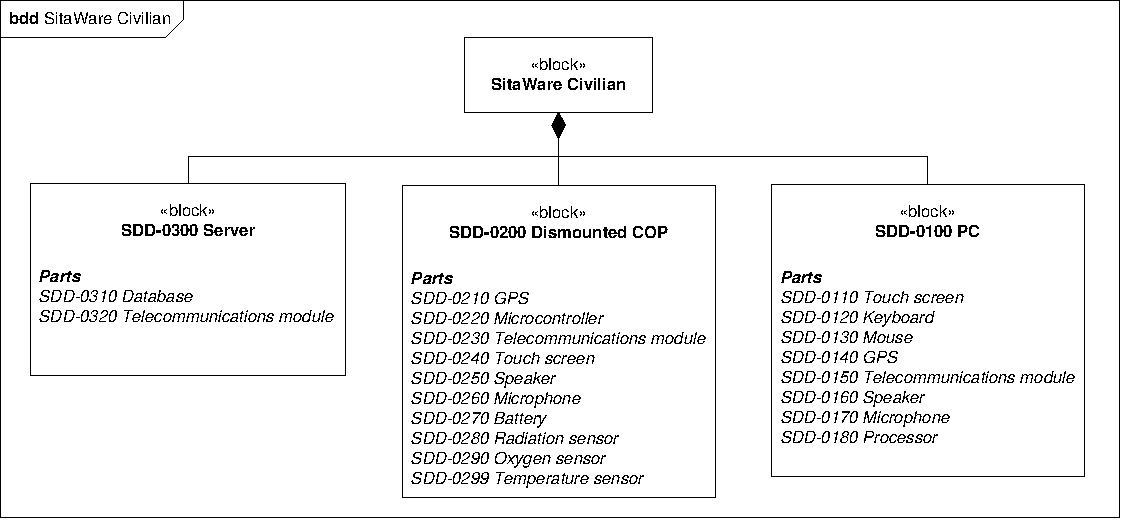
\includegraphics[width=0.95\textwidth]
{billeder/bdd_overordnet.pdf}
\caption{Block diagram of the system.}
\label{fig:block_diagram}
\end{figure}
The diagram consists of system-blocks along with parts associated to each block. The system-blocks are depicted as two-compartment blocks with the name of the block in the first compartment, and sub parts in the second compartment. In the next section, a short description of each system-block is given.
\subsection{Component description}
\begin{enumerate}
\item[•] \textbf{PC:} This block constitutes the machine in the head quarter (HQ) on which the COP-software will be executed. It is not within the scope of this project to develop the PC itself. However, there are parts required for the PC to enable it to interact with the rest of the system. These parts are specified in the block diagram. The PC has a GPS module, so that the location of the HQ is always known. The PC also has a telecommunication module, in order to be able to communicate with the rest of the system. Furthermore the PC has a touchscreen that lets the user navigate in the application through touch inputs. An audio interface is constituted of a microphone and a speaker.
\item[•] \textbf{Server:} The server will facilitate communication between the other blocks. It has a telecommunication module, in order to be able to communicate with the rest of the system. In addition, it will store user information along with logs locally in an internal database.
\item[•] \textbf{Dismounted COP:} This block constitutes the machine on which the condensed COP-software will be executed. The dismounted COP will be used by the dismounted users in the field. It has a GPS module, so that the location of the dismounted users is always known. Furthermore it has a telecommunication module so that it will be able to communicate with the rest of the system. Furthermore the dismounted COP has a touchscreen that lets the user navigate in the application through touch inputs. An audio interface is constituted of a microphone and a speaker. Lastly the dismounted COP has a radioation sensor, an oxygen sensor and a temperature sensor to enable detection of radiation-, oxygen-, and temperature-levels. 
\end{enumerate}

\section{Concept of execution}

\begin{figure}[H]
\centering
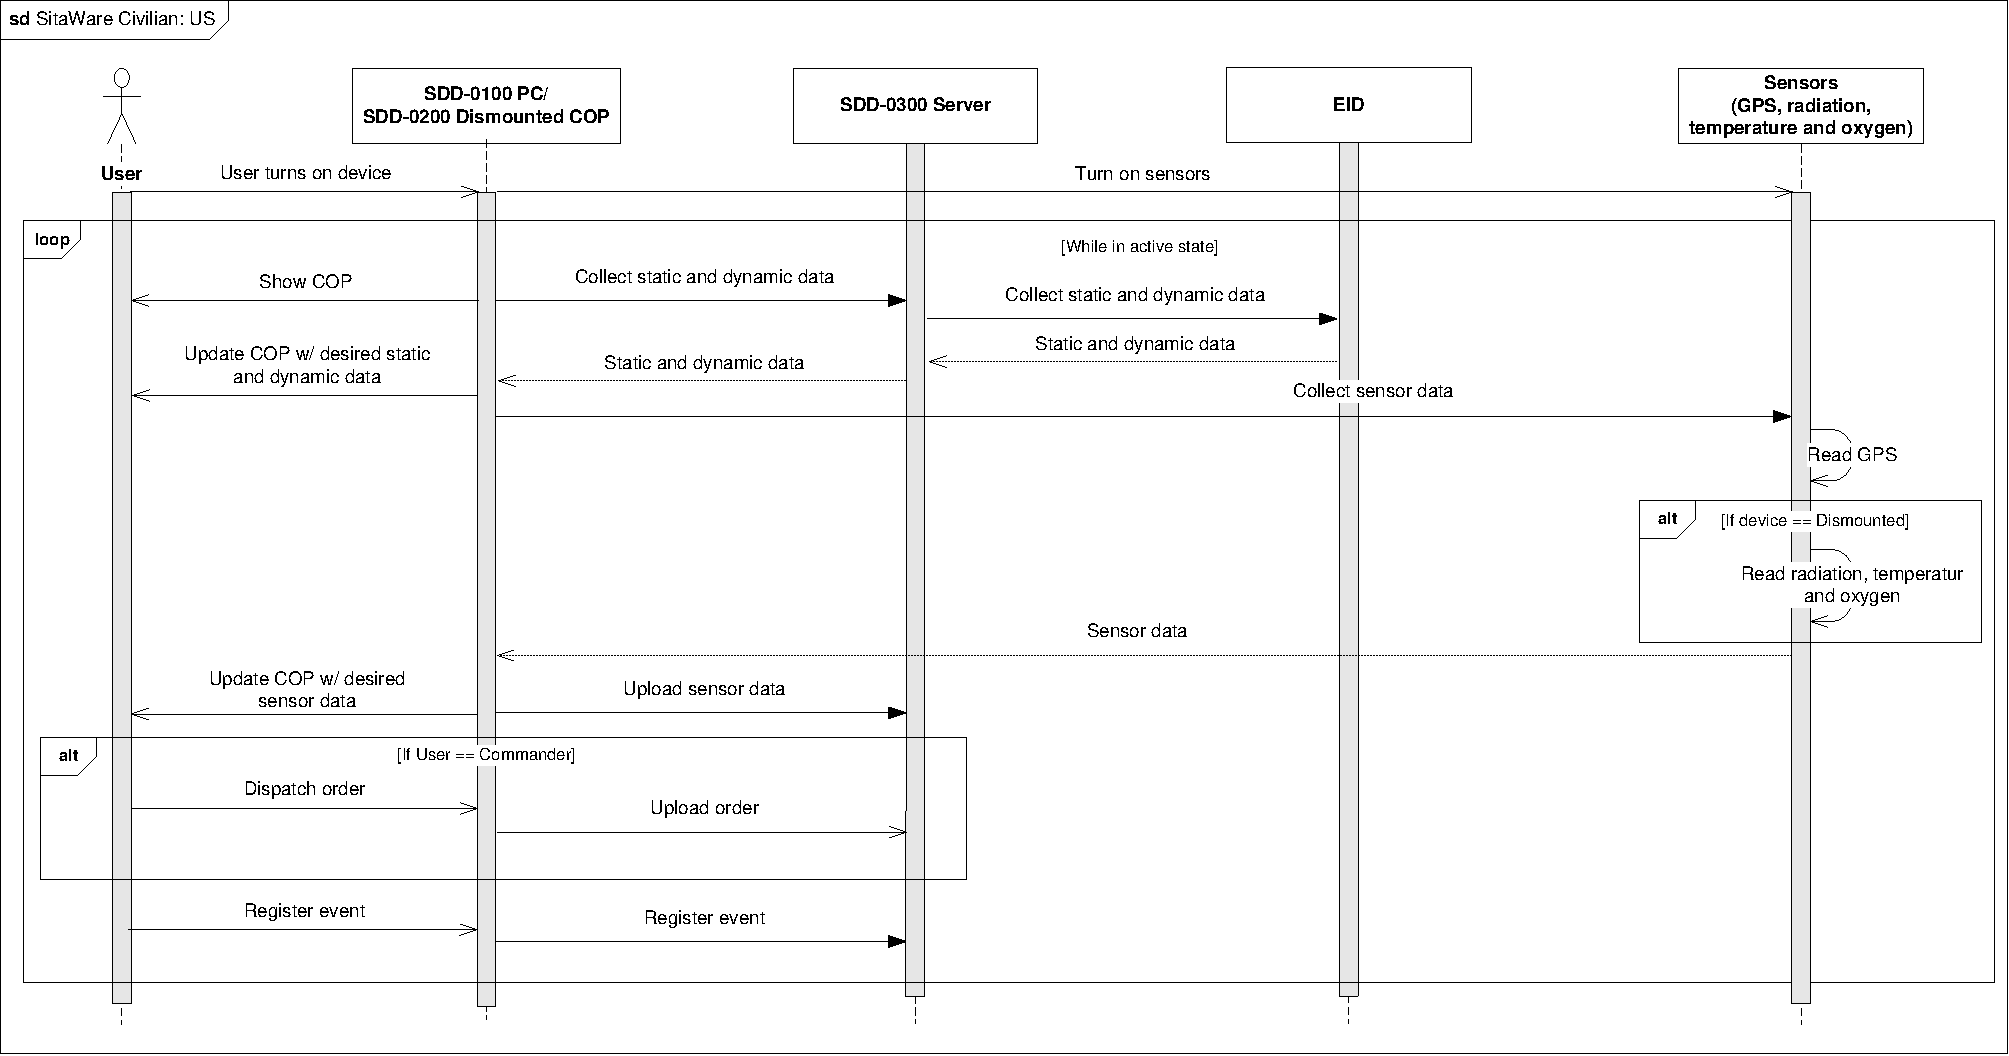
\includegraphics[width=0.95\textwidth]
{billeder/sekvens1.pdf}
\caption{Overall sequence diagram for SitaWare Civilian.}
\label{fig:sekvens1}
\end{figure}

\section{Interface Design}

This section seeks to describe the interface characteristics of the system components. It provides an internal block diagram (bdd) of the system, where the interfaces of the system components are identified, as long as the external interfaces of the system. The internal block diagram of the overall system is shown in figure \ref{fig:internal_block_diagram}:
\begin{figure}[H]
\centering
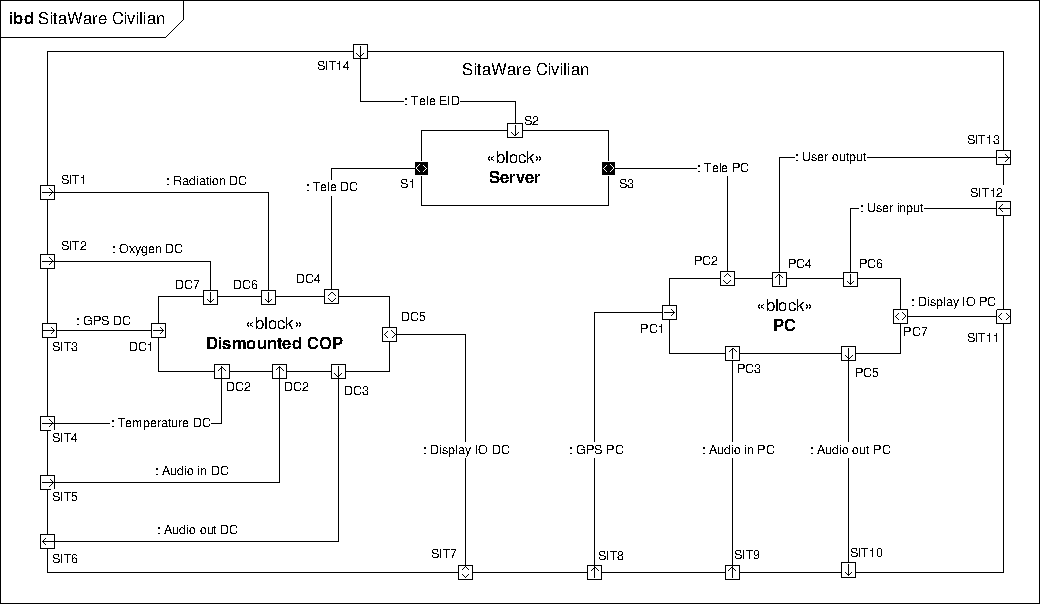
\includegraphics[width=0.95\textwidth]
{billeder/ibd_overordnet.pdf}
\caption{Internal block diagram of the system.}
\label{fig:internal_block_diagram}
\end{figure}


\begin{table}[H]  
\centering

\begin{tabular}{|l|p{8cm}|l|l|} 
\hline
	\textbf{Name}		& \textbf{Description}						  & \textbf{Port 1} & \textbf{Port 2} \\\hline
  Radiation DC				&  Radiation level to the dismounted COP 	 					   & SIT1 & DC6 \\\hline
  Oxygen DC					&  Oxygen level signal to the dismounted COP				   & SIT2 & DC7 \\\hline
  GPS DC					&  GPS signal for the dismounted COP 	 					   & SIT3 & DC1 \\\hline   
  Temperature DC			&  Temperature signal to the dismounted COP 	 					   & SIT4 & DC2 \\\hline     
  Audio in DC				&  Microphone for communication purposes 	 				   & SIT5 &DC8\\\hline     
  Audio out DC				&  Speaker for communication purposes 	 					   & SIT6 & DC3 \\\hline     
  Display IO DC				&  Display input/output for dismounted COP 	 					   & SIT7 & DC5 \\\hline     
  
  GPS PC					&  GPS signal for the PC			 	 					   & SIT8 & PC1 \\\hline     
  Audio in PC				&  Microphone for communication purposes 	 					   & SIT9 & PC3 \\\hline     
  Audio out PC				&  Speaker for communication purposes 	 					   & SIT10 & PC5 \\\hline     
  Display IO PC				&  Display input/output for PC 	 					   & SIT11 & PC7 \\\hline     
  Keyboard PC				&  Keyboard input to the PC 	 					   & SIT12 & PC6 \\\hline     
  Mouse in PC				&  Mouse input to the PC 	 					   & SIT13 & PC4 \\\hline    
  Tele EID S				&  Telecommunication between the server, and an external information database				   & SIT14 & S2 \\\hline
       
  Tele DC					&  Telecommunication between the dismounted COP and the server & DC4 & S1 \\\hline   
  Tele 						&  Telecommunication between the PC and the server 					   & PC2 & S2 \\\hline   
   
\end{tabular}
\caption {General ibd} 
%\label{} 
\end{table} 




\subsection{PC}
In this section the internal interfaces of the PC to be used in this system are specified in greater detail. All the sub parts of the PC are connected to the processor which manages all logic operations and functions, while the telecommunication module enables the PC to communicate with the remaining system components. It is not within the scope of this project to develop the PC itself, however the COP is to be executed on the PC. Therefore the interfaces of the PC are identified, to ensure that the PC - and thereby the COP - can communicate with the rest of the system. The internal block diagram of the PC is shown in figure \ref{fig:internal_diagram_PC}:
\begin{figure}[H]
\centering
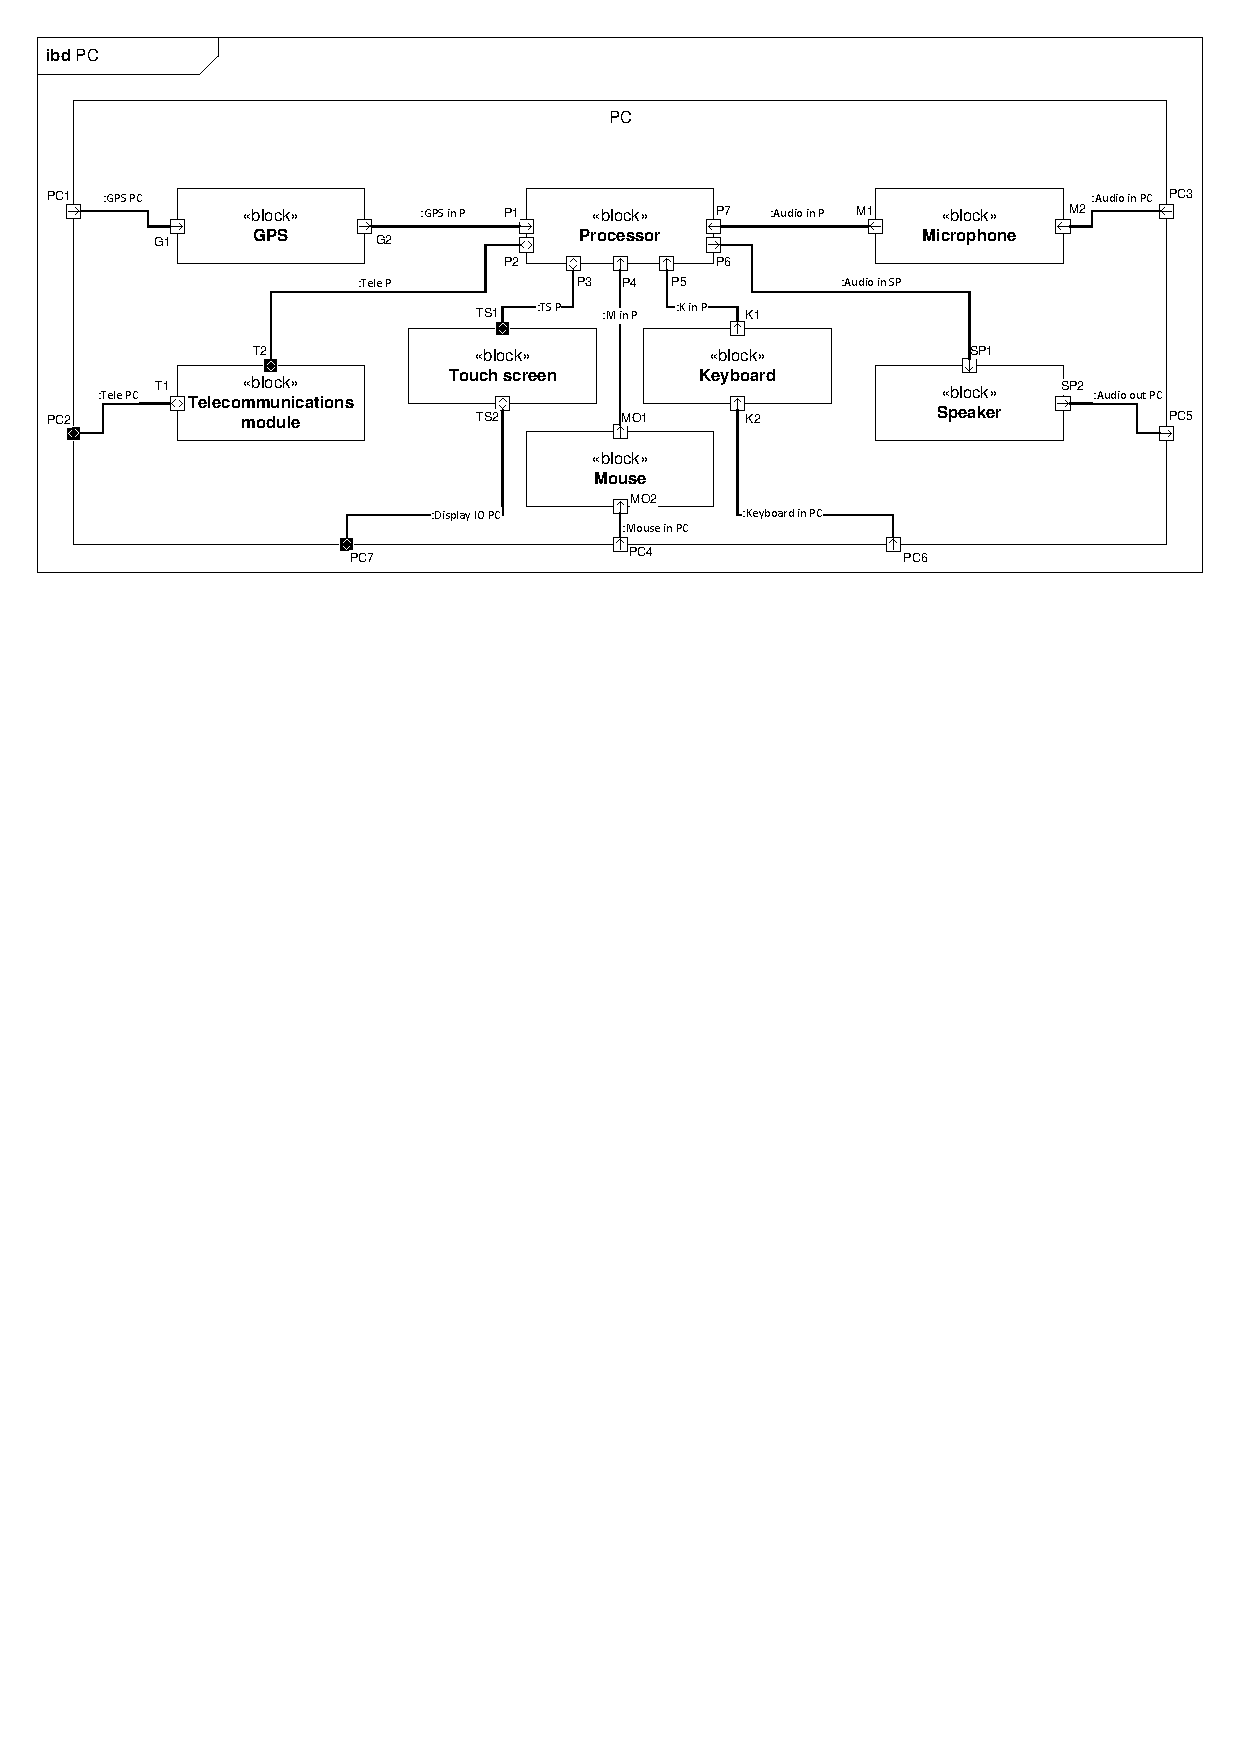
\includegraphics[width=0.95\textwidth]
{billeder/ibd_PC.pdf}
\caption{Internal block diagram of the PC.}
\label{fig:internal_diagram_PC}
\end{figure}


\begin{table}[H]  
\centering

\begin{tabular}{|l|p{8cm}|l|l|} 
\hline
	\textbf{Name}		& \textbf{Description} & \textbf{Port 1} & \textbf{Port 2} \\\hline
GPS DC	    & Dismounted COP receiving GPS signal												 & G1 &  PC1 \\\hline
Tele PC     & Telecommunication between the PC and the server							   		 & T1 &  PC2 \\\hline		
Audio in PC & Microphone for communication purposes  											 & M2 &  PC3 \\\hline				  
Mouse in PC	    & Input from the mouse										 					 & MO2 &  PC4\\\hline				  
Audio out PC	        & Speaker for communication purposes 			  						 & SP2 & PC5 \\\hline			
Keyboard in PC	& Input from the keyboard   				 				 					 & K2 &  PC6 \\\hline				  
Display IO PC	& Input and output from user to the touch screen								 & TS2 &  PC7 \\\hline				  
	
GPS in P	& Signal from the GPS to the processor								                 & P1 & G2 \\\hline				  			
Tele P		& Communication between the telecommunications module and the processor              & P2 & T2 \\\hline				  			
TS P		& Communication between the touch screen module and the processor          			 & P3 & TS1 \\\hline			  			
M in P		& Signal from the mouse to the processor          								     & P4 & MO1 \\\hline				  	
K in P		& Signal from the keyboard to the processor          								 & P5 & K1 \\\hline				  			
Audio in SP	& Signal from the processor to the speaker					             			 & P6 & SP1 \\\hline				  		Audio in P	& Signal from the microphone to the processor					           		     & P7 & M1 \\\hline				  			
												   
\end{tabular}
\caption {Dismounted COP ibd} 
%\label{} 
\end{table} 


\chapter{Requirements traceability}
\label{chap:req_trace}
This chapter traces the requirements to the user needs.

\section{Traceability matrix}
The traceability matrix ensures that all requirements fulfill a need. If a requirement does not fulfill a need, then it is redundant, or a new need has to be created.
In the context of the detailed design description, a reference to the unique names of blocks and states has been added to the corresponding requirements in the "Design document reference" column of the traceability matrix. 

\begin{sidewaystable}
\begin{table}[H]
\begin{tabular}{|l|l|l|l|}
\hline
 \textbf{Project name:} & SitaWare Civilian & \textbf{Business area:}  & Civilian Crises Management\\ \hline
 \textbf{Project manager:} & René Arendt Sørensen & \textbf{Business Analyst lead:} & Rasmus Fredensborg Jensen\\ \hline
 \textbf{QA lead} & Peter Kristian Mathiesen & \textbf{Target implementation date:}  & \\ \hline
\end{tabular}	
\begin{tabular}{|p{2cm}|p{2cm}|p{3cm}|p{2cm}|p{2cm}|p{2cm}|p{2cm}|p{2cm}|p{2cm}|}
\hline
 Req. id. & Catagory of functional activity & Requirement description  & Use case reference & Design document reference & Code or module reference & Test case reference & User acceptance validation & Comments\\ \hline
 FR-0030 & & States & &SM-0100  & & ST-0010 & &\\ \hline 
FR-0040 & & States & &SM-0200 & & ST-0020& &\\ \hline  
FR-0050 & & States & &SM-0300 & & ST-0030 & &\\ \hline  
FR-0060 & & States & &SM-0400 & & ST-0040& &\\ \hline  
FR-0070 & & Modes & &SM-0210 & & ST-0050& &\\ \hline  
FR-0080 & & Modes & &SM-0220 & & ST-0060& &\\ \hline 
FR-0090 & & Modes & &SM-0230 & & ST-0070& &\\ \hline 
 FR-0110 & N-030 & Capability & &SDD-0210, SDD-0140 & & ST-0105& &\\ \hline
 FR-0115 & N-020 & Capability & &SDD-0110, SDD-0150, SDD-0240, SDD-0230, SDD-0300, SDD-0320& & ST-0110& &\\ \hline
 FR-0120 & N-020 & Capability & &SDD-0300, SDD-0320 & & ST-0115& &\\ \hline
 FR-0130 & N-020 & Capability & &SDD-0300, SDD-0320 & & ST-0120& &\\ \hline
 FR-0140 & N-020 & Capability & &SDD-0300, SDD-0320 & & ST-0125& &\\ \hline
 FR-0150 & N-020 & Capability & &SDD-0300, SDD-0320& & ST-0130& &\\ \hline
\end{tabular}	
\caption{Requirement traceability matrix.}
\end{table}

\end{sidewaystable}

\begin{sidewaystable}
\begin{table}[H]
\begin{tabular}{|l|l|l|l|}
\hline
 \textbf{Project name:} & SitaWare Civilian & \textbf{Business area:}  & Civilian Crises Management\\ \hline
 \textbf{Project manager:} & René Arendt Sørensen & \textbf{Business Analyst lead:} & Rasmus Fredensborg  Jensen\\ \hline
 \textbf{QA lead} & Peter Kristian Mathiesen & \textbf{Target implementation date:}  & \\ \hline
\end{tabular}	
\begin{tabular}{|p{2cm}|p{2cm}|p{3cm}|p{2cm}|p{2cm}|p{2cm}|p{2cm}|p{2cm}|p{2cm}|}
\hline
 Req. id. & Catagory of functional activity & Requirement description  & Use case reference & Design document reference & Code or module reference & Test case reference & User acceptance validation & Comments\\ \hline
  FR-0160 & N-020 & Capability & &SDD-0300, SDD-0320 & & ST-0135& &\\ \hline
 FR-0170 & N-010 & Capability & &SDD-0150, SDD-0230, SDD-0310, SDD-0320 & & ST-0140& &\\ \hline 
 FR-0180 & N-020 & Capability & &SDD-0150, SDD-0230, SDD-0310, SDD-0320  & & ST-0145& &\\ \hline
 FR-0190 & N-020 & Capability & &SDD-0110, SDD-0240 & & ST-0150& &\\ \hline
 FR-0200 & N-020 & Capability & &SDD-0110,  SDD-0150, SDD-0230, SDD-0240, SDD-0310, SDD-0320& & ST-0155& &\\ \hline 
\end{tabular}	
\caption{Requirement traceability matrix.}
\end{table}

\end{sidewaystable}



\begin{sidewaystable}
\begin{table}[H]
\begin{tabular}{|l|l|l|l|}
\hline
 \textbf{Project name:} & SitaWare Civilian & \textbf{Business area:}  & Civilian Crises Management\\ \hline
 \textbf{Project manager:} & René Arendt Sørensen & \textbf{Business Analyst lead:} & Rasmus Fredensborg  Jensen\\ \hline
 \textbf{QA lead} & Peter Kristian Mathiesen & \textbf{Target implementation date:}  & \\ \hline
\end{tabular}	
\begin{tabular}{|p{2cm}|p{2cm}|p{3cm}|p{2cm}|p{2cm}|p{2cm}|p{2cm}|p{2cm}|p{2cm}|}
\hline
 Req. id. & Catagory of functional activity & Requirement description  & Use case reference & Design document reference & Code or module reference & Test case reference & User acceptance validation & Comments\\ \hline
 FR-0210 & N-020 & Capability & &SDD-0110,  SDD-0150, SDD-0230, SDD-0240, SDD-0310, SDD-0320& & ST-0160& &\\ \hline
 FR-0220 & N-010 & Capability & &SDD-0330 & & ST-0165& &\\ \hline
 FR-0230 & N-020 & Capability & &SDD-0140, SDD-0150, SDD-0210, SDD-0230, SDD-0310, SDD-0320& & ST-0170& &\\ \hline
 FR-0240 & N-020 & Capability & &SDD-0150, SDD-0230, SDD-0310, SDD-0320& & ST-0175& &\\ \hline
 FR-0250 & N-020 & Capability & &SDD-0150, SDD-0230, SDD-0310, SDD-0320 & & ST-0180& &\\ \hline
 FR-0260 & N-020 & Capability & &SDD-0150, SDD-0230, SDD-0310, SDD-0320 & & ST-0185& &\\ \hline

\end{tabular}	
\caption{Requirement traceability matrix.}
\end{table}

\end{sidewaystable}

\begin{sidewaystable}
\begin{table}[H]
\begin{tabular}{|l|l|l|l|}
\hline
 \textbf{Project name:} & SitaWare Civilian & \textbf{Business area:}  & Civilian Crises Management\\ \hline
 \textbf{Project manager:} & René Arendt Sørensen & \textbf{Business Analyst lead:} & Rasmus Fredensborg  Jensen\\ \hline
 \textbf{QA lead} & Peter Kristian Mathiesen & \textbf{Target implementation date:}  & \\ \hline
\end{tabular}	
\begin{tabular}{|p{2cm}|p{2cm}|p{3cm}|p{2cm}|p{2cm}|p{2cm}|p{2cm}|p{2cm}|p{2cm}|}
\hline
 Req. id. & Catagory of functional activity & Requirement description  & Use case reference & Design document reference & Code or module reference & Test case reference & User acceptance validation & Comments\\ \hline
  FR-0270 & N-010 & External interface & &SDD-110, SDD-0240& & ST-0210 & &\\ \hline
 FR-0280 & N-010 & External interface & &SDD-110, SDD-0240 & & ST-0220 & &\\ \hline
 FR-0290 & N-010 & External interface & &SDD-0160, SDD-0170, SDD-0250, SD-0260& & ST-0230 & &\\ \hline
 FR-0300 & N-020 & External interface & &SDD-0150, SDD-0230, SDD-0300, SDD-0310, SDD-0320& & ST-0240 & &\\ \hline
 FR-0320 & N-010 & Internal interface & &SDD-0150, SDD-0230, SDD-0320& & ST-0310 & &\\ \hline
 FR-0330 & & Data interface & &SDD-0310 & & ST-0410 & &\\ \hline
 FR-0340 & & Data interface & &SDD-0310 & & ST-0420 & &\\ \hline
 FR-0350 & N-020 & Safety & &SDD-0280 & & ST-0510 & &\\ \hline
 FR-0352 & N-020 & Safety & &SDD-0299 & & ST-0520 & &\\ \hline 
 FR-0354 & N-020 & Safety & &SDD-0290 & & ST-0530 & &\\ \hline

 
\end{tabular}	
\caption{Requirement traceability matrix.}
\end{table}

\end{sidewaystable}






\begin{sidewaystable}
\begin{table}[H]
\begin{tabular}{|l|l|l|l|}
\hline
 \textbf{Project name:} & SitaWare Civilian & \textbf{Business area:}  & Civilian Crises Management\\ \hline
 \textbf{Project manager:} & René Arendt Sørensen & \textbf{Business Analyst lead:} & Rasmus Fredensborg  Jensen\\ \hline
 \textbf{QA lead} & Peter Kristian Mathiesen & \textbf{Target implementation date:}  & \\ \hline
\end{tabular}	
\begin{tabular}{|p{2cm}|p{2cm}|p{3cm}|p{2cm}|p{2cm}|p{2cm}|p{2cm}|p{2cm}|p{2cm}|}
\hline
 Req. id. & Catagory of functional activity & Requirement description  & Use case reference & Design document reference & Code or module reference & Test case reference & User acceptance validation & Comments\\ \hline
  FR-0360 & & Security & &SDD-0110, SDD-0240 & & ST-0610 & &\\ \hline
 FR-0370 & & Security & && & ST-0620 & &\\ \hline   	
 FR-0380 & & Security & && & ST-0630 & &\\ \hline
 FR-0390 & & Environment & && &ST-0710 & &\\ \hline
 FR-0400 & & Environment & && &ST-0720 & &\\ \hline
 FR-0410 & & Environment & && &ST-0730 & &\\ \hline
 FR-0420 & & Environment & && &ST-0740 & &\\ \hline
 FR-0430 & N-040 & Quality & && &ST-0810 & &\\ \hline
 FR-0440 & & Quality & && &ST-0820 & &\\ \hline
 FR-0450 & & Quality & && &ST-0830 & &\\ \hline
 FR-0460 & & Design constraints & && &ST-0910 & &\\ \hline
 FR-0470 & & Design constraints & && &ST-0920 & &\\ \hline
 FR-0480 & & Personnel-related & && &ST-1010 & &\\ \hline 
\end{tabular}	
\caption{Requirement traceability matrix.}
\end{table}

\end{sidewaystable}



\begin{sidewaystable}
\begin{table}[H]
\begin{tabular}{|l|l|l|l|}
\hline
 \textbf{Project name:} & SitaWare Civilian & \textbf{Business area:}  & Civilian Crises Management\\ \hline
 \textbf{Project manager:} & René Arendt Sørensen & \textbf{Business Analyst lead:} & Rasmus Fredensborg  Jensen\\ \hline
 \textbf{QA lead} & Peter Kristian Mathiesen & \textbf{Target implementation date:}  & \\ \hline
\end{tabular}	
\begin{tabular}{|p{2cm}|p{2cm}|p{3cm}|p{2cm}|p{2cm}|p{2cm}|p{2cm}|p{2cm}|p{2cm}|}
\hline
 Req. id. & Catagory of functional activity & Requirement description  & Use case reference & Design document reference & Code or module reference & Test case reference & User acceptance validation & Comments\\ \hline
 NFR-0100 &  & Non-functional & & & & ST-1110 & &\\ \hline
 NFR-0110 &  & Non-functional & & & & ST-1120 & &\\ \hline
 NFR-0120 &  & Non-functional & & & & ST-1130 & &\\ \hline
 NFR-0130 &  & Non-functional & & & & ST-1140 & &\\ \hline
 NFR-0140 &  & Non-functional & & & & ST-1150 & &\\ \hline
 NFR-0150 &  & Non-functional & & & & ST-1160 & &\\ \hline
 NFR-0160 &  & Non-functional & & & & ST-1170 & &\\ \hline
 NFR-0170 &  & Non-functional & & & & ST-1180 & &\\ \hline
 NFR-0180 &  & Non-functional & & & & ST-1190 & &\\ \hline
 NFR-0190 &  & Non-functional & & & & ST-1200 & &\\ \hline
 NFR-0200 &  & Non-functional & & & & ST-1210 & &\\ \hline
 NFR-0210 &  & Non-functional & & & & ST-1220 & &\\ \hline
\end{tabular}	
\caption{Requirement traceability matrix.}
\end{table}

\end{sidewaystable}


%%%% Fixme-listen %%%%
%\newpage										% Ny side til Fixme-listen
%\listoffixmes									% Fixme-listen - fjernes til sidst i projektet med "%"



\end{document}									% Slutter dokumentet - obligatorisk